\section{Technologien}

\subsection{Technologie Versionen}

\subsubsection{Technologie Liste}

\begin{center}
\begin{tabular}{|c|c|}
\hline

\includegraphics[width=0.15\textwidth]{bilder/technologien/NodeJS.png} &
\multirow[c]{1}[1]{*}[30pt]{Node.js 14.18.0 LTS} \\
\hline

\includegraphics[width=0.15\textwidth]{bilder/technologien/Angular.png} &
\multirow[c]{1}[1]{*}[30pt]{Angular 12.2.9} \\
\hline

\includegraphics[width=0.15\textwidth]{bilder/technologien/Socket.io.png} &
\multirow[c]{1}[1]{*}[30pt]{Socket.io 4.2.0} \\
\hline

\includegraphics[width=0.15\textwidth]{bilder/technologien/mongoDB.png} &
\multirow[c]{1}[1]{*}[30pt]{MongoDB Community Edition 5.0.3} \\
\hline

\includegraphics[width=0.15\textwidth]{bilder/technologien/KeyCloak.png} &
\multirow[c]{1}[1]{*}[30pt]{KeyCloak 15.0.2} \\
\hline
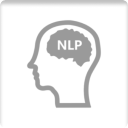
\includegraphics[width=0.15\textwidth]{bilder/technologien/NLP.png} &
\multirow[c]{1}[1]{*}[30pt]{NLP.js 4.22.2 (optional)} \\
\hline
\end{tabular}
\end{center}

\subsubsection{Entscheidung für die Technologien}
Bei der Wahl der Technologien haben wir nach Möglichkeit LTS Versionen gesucht.
Damit wir eine Applikation erstellen können, die für lange Zeit Sicherheitsupdates
bekommt. Zusätzlich haben wir als Ziel, dass die Software als ingesamtes Paket sehr lange
stabil läuft und dadurch Ausfälle minimiert werden.

\subsubsection{NLP.js 4.22.2 (optional)}
Damit wir NLP.js nutzen können benötigen wir eine LTS Version von Node.js.
Diese Begrenzung haben wir zusätzlich in die Technologie Entscheidung einbezogen.
Damit die Integration von NLP.js in den Chatbot später immernoch möglich ist.

\subsection{Technologie Vergleich}
\subsubsection{Angular vs Vue.js}

\begin{center}
\begin{tabular}{|p{0.25\linewidth}|p{0.33\linewidth}|p{0.33\linewidth}|}
\hline
\textbf{} & \textbf{Angular} & \textbf{Vue.js} \\
\hline
\textbf{Framework,\newline Library, Platform} & Entwicklungsplattform\newline (Development platform) & Progressive Framework \\
\hline
\textbf{Gründer} & Google & ehemaliger Google\newline Mitarbeiter \\
\hline
\textbf{Technology Typ} & MVC Framework & MVVM Framework \\
\hline
\textbf{Programmier-\newline sprache} & TypeScript & JavaScript \\
\hline
\textbf{Performance} & niedrig & hoch \\
\hline
\textbf{Größe} & 500 kB & 80 kB \\
\hline
\textbf{Lernkurve} & Eine steile Lernkurve & Eine geringe Lernkurve \\
\hline
\textbf{Dokumentation} & vorhanden & vorhanden \\
\hline
\textbf{Datenbindung} & Bi-directional & Bi-directional \\
\hline
\textbf{Rendering} & beim Client & beim Server \\
\hline
\textbf{Code reuse} & möglich & Ja, CSS und HTML \\
\hline
\textbf{Skalierbarkeit} & sehr hoch & hoch \\
\hline
\textbf{Testbarkeit} & mit einem Tool & mehrere Tools benötigt \\
\hline
\textbf{Vollständige Web\newline App} & Kann als standalone Basis verwendet werden & benötigt Third Party Tools \\
\hline
\textbf{Lizenz} & MIT License & MIT License \\
\hline
\end{tabular}
\end{center}

\subsubsection{MongoDB vs PostgreSQL}

\begin{center}
\begin{tabular}{|p{0.25\linewidth}|p{0.33\linewidth}|p{0.33\linewidth}|}
\hline
\textbf{} & \textbf{MongoDB} & \textbf{PostgreSQL} \\
\hline
\textbf{Primäres\newline Datenbankmodell} & Dokumentation & Relationales DBMS \\
\hline
\textbf{Entwickler} & MongoDB. Inc & PostgreSQL Global\newline Development Group \\
\hline
\textbf{Datenschema} & Schemafrei (NoSQL) & Ja \\
\hline
\textbf{Programmier-\newline sprachen} & JavaScript + 28 weitere & JavaScript + 9 weitere \\
\hline
\textbf{Query Language} & MQL & SQL \\
\hline
\textbf{Maximale\newline Dateigröße} & 16 MB & 1 GB \\
\hline
\textbf{Lernkurve} & Eine geringe Lernkurve & Eine geringe Lernkurve \\
\hline
\textbf{Dokumentation} & vorhanden & vorhanden \\
\hline
\textbf{Skalierbarkeit} & sehr hoch & hoch \\
\hline
\textbf{Lizenz} & Open Source & Open Source \\
\hline
\end{tabular}
\end{center}

\subsection{Technologie Diagramme}
 Hier werden die Zusammenhänge der Technologien in Form von verschiedenen Diagrammen vorgestellt.

\subsubsection{Komponentendiagramme}

\begin{figure}[!hbt]
\centering
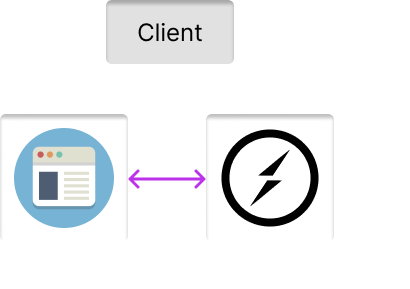
\includegraphics[width=0.5\textwidth]{bilder/technologien/KomponentendiagramClient.png}
\caption{Komponentendiagramm Client}
\label{fig:Komponentendiagramm_Client}
\end{figure}
Hier wird die Client Seite bildlich dargestellt. Man sieht, dass der Webbrowseer durch die 
Socket.io Client deployed wird und dadurch wird dann eine Beziehung zur Serverseite auifgebaut (siehe Abbildung 2).

\begin{figure}[!hbt]
\centering
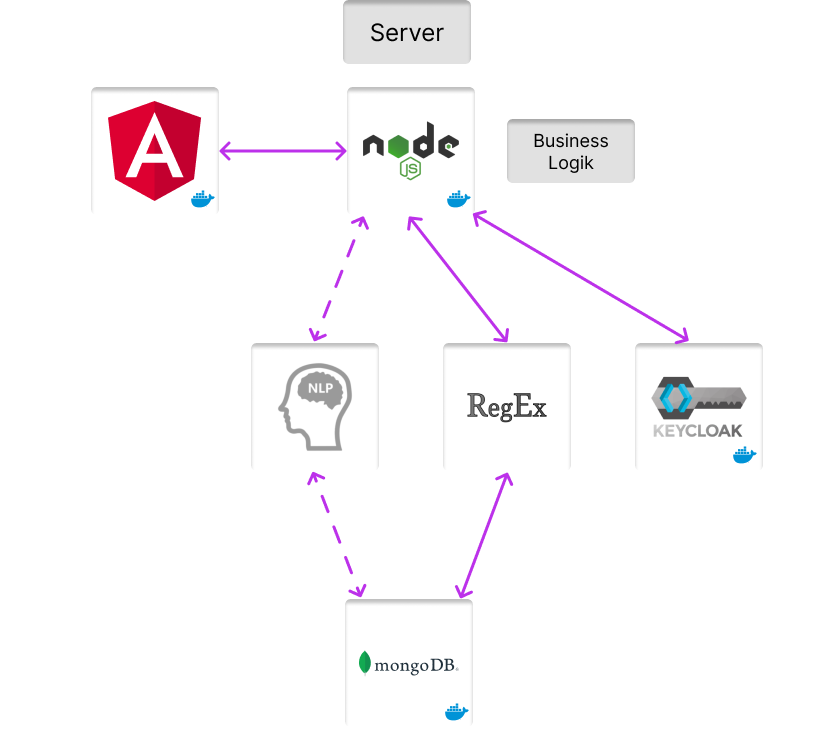
\includegraphics[width=0.9\textwidth]{bilder/technologien/KomponentendiagramServer.png}
\caption{Komponentendiagramm Server}
\label{fig:Komponentendiagramm_Server}
\end{figure}
In der Serverseite wird dann durch den Socket.io Server die Verbindug zum Clienten aufrecht gehalten.
Im Server befindet sich Angular, node.js, KeyCloak und die Datenbank mongoDB und haben jeweils einen eigenen Dockercontainer. 
Die Erkennung von der eingegeben Sprache möchten wir zunächst mit RegEx ermöglichen, 
um das Minimal Virable Product hinzubekommen. Optional dann mit NLP (Natural Language Processing) erweitern.

\begin{figure}[!hbt]
\centering
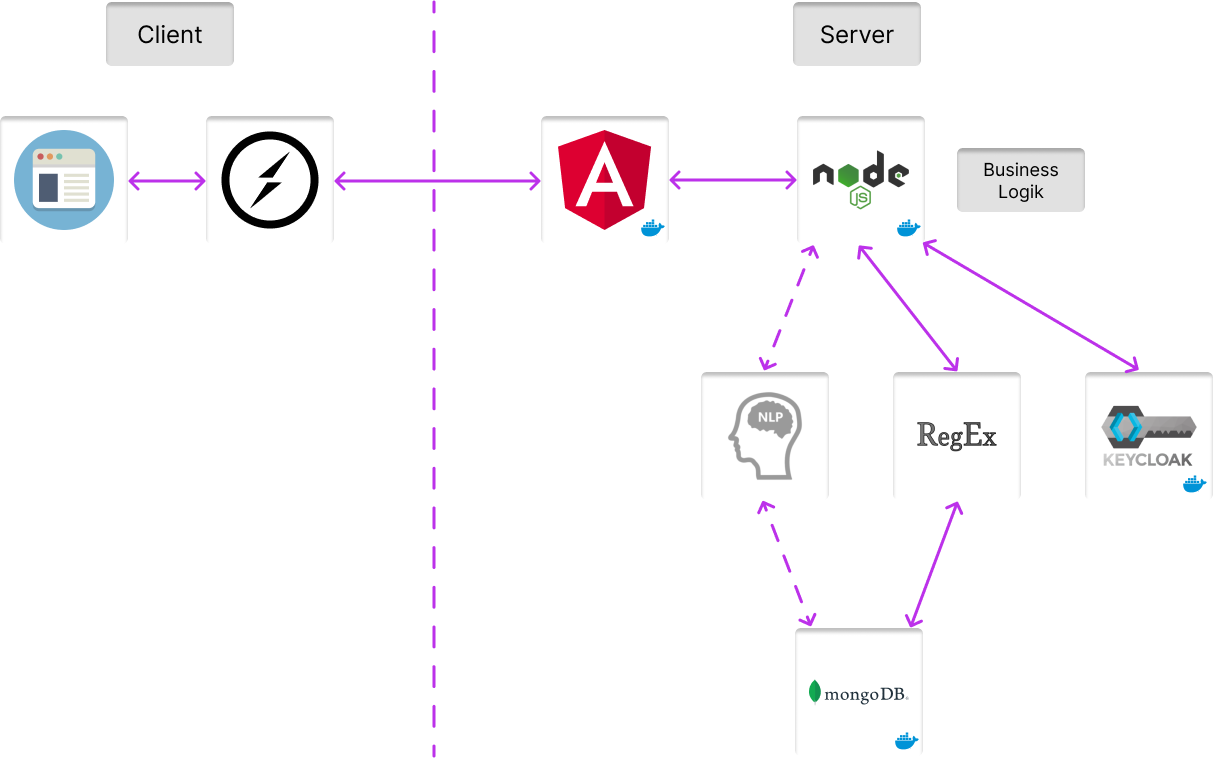
\includegraphics[width=1.0\textwidth]{bilder/technologien/Komponentendiagram v1.2.png}
\caption{Komponentendiagramm v1.2}
\label{fig:Komponentendiagramm_v1.2}
\end{figure}

\begin{figure}
\centering
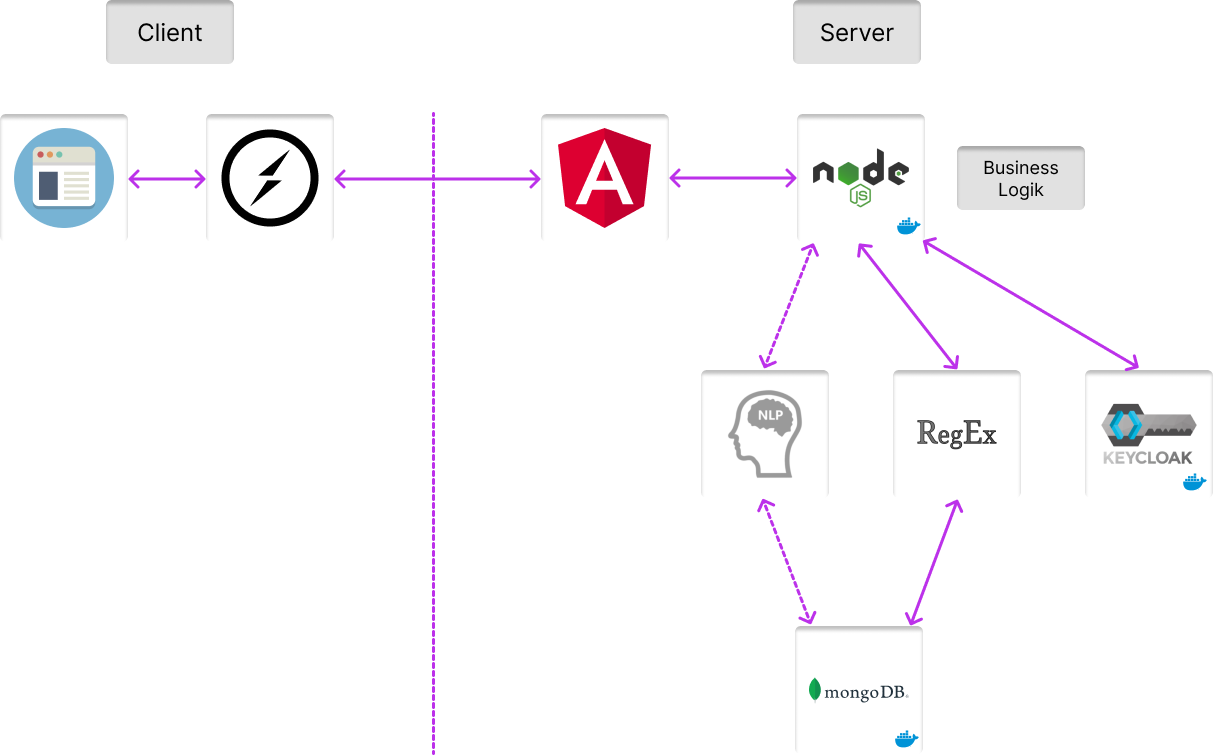
\includegraphics[width=1.0\textwidth]{bilder/technologien/Komponentendiagram v1.1.png}
\caption{Komponentendiagramm v1.1}
\label{fig:Komponentendiagramm_v1.1}
\end{figure}

\begin{figure}
\centering
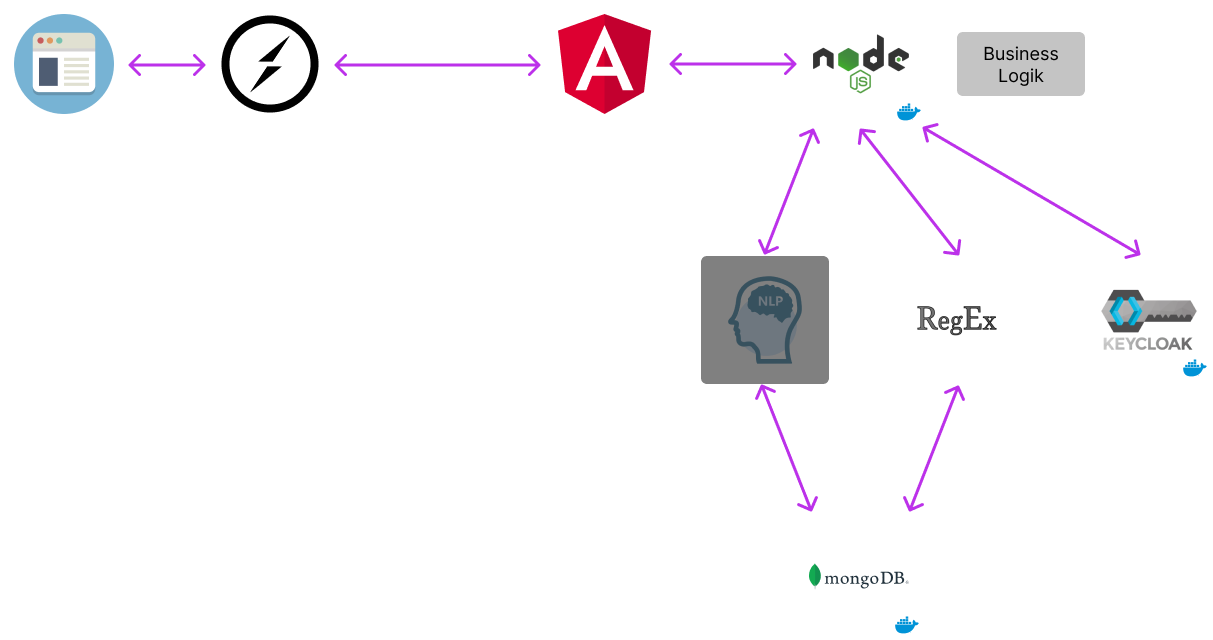
\includegraphics[width=1.0\textwidth]{bilder/technologien/Komponenten-Diagram-v1.png}
\caption{Komponentendiagramm v1.0}
\label{fig:Komponentendiagramm_v1.0}
\end{figure}
\FloatBarrier % prevent pictures from appearing under a different section